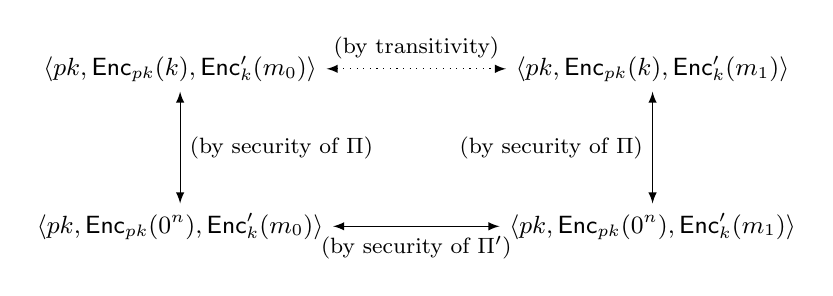
\begin{tikzpicture}[font=\small]
\node (pk0) at (0,0) {$\langle pk,\mathsf{Enc}_{pk}(k),\mathsf{Enc}_{k}'(m_0)\rangle$};
\node (pk1) at (6,0) {$\langle pk,\mathsf{Enc}_{pk}(k),\mathsf{Enc}_{k}'(m_1)\rangle$};
\node (k0) at (0,-2) {$\langle pk,\mathsf{Enc}_{pk}(0^n),\mathsf{Enc}_{k}'(m_0)\rangle$};
\node (k1) at (6,-2) {$\langle pk,\mathsf{Enc}_{pk}(0^n),\mathsf{Enc}_{k}'(m_1)\rangle$};
\draw[latex-latex,dotted] (pk0) -- (pk1) node [midway,above] {\footnotesize (by transitivity)};
\draw[latex-latex] (k0) -- (k1) node [midway,below] {\footnotesize (by security of $\Pi'$)};
\draw[latex-latex] (pk0) -- (k0) node [midway,right] {\footnotesize (by security of $\Pi$)};
\draw[latex-latex] (pk1) -- (k1) node [midway,left] {\footnotesize (by security of $\Pi$)};
\end{tikzpicture}